\section {Design and Implementation\\}

\subsection{Reactor Model\\}
The PushUp Server runs atop of the Twisted framework\cite{Twisted}, which 
adopts the reactor model\cite{Reactor} to enable event-driven mechanism.

The reactor manages how to register handlers for particular event types, and 
how to activate event handlers as events occur within a single thread. 
Moreover the reactor can manages multiple event-loops without introducing 
additional threads. 

Figure \ref{fig:eventloop} demonstrates the how the execution switches
between the event loops and user code. Figure \ref{fig:eventloop_flow} 
further illustrates the detailed work flow.

The reactor has well encapsulated the operating systems' underlying 
event notification mechanism (normally it is kqueue() in Unix and 
epoll() in Linux) and presents a convenient programming interface
for the developers.

\begin{figure}[htb!]
    \centering%
    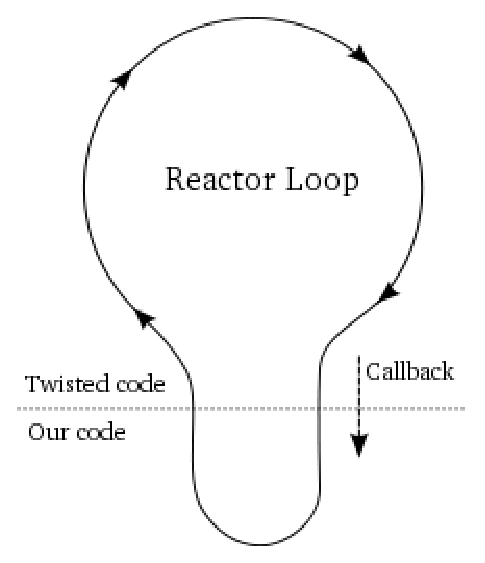
\includegraphics[scale=0.70]{figures/mainloop.eps}
    \caption{Work flow of Twisted Reactor Model}
    \label{fig:mainloop}
\end{figure}
\begin{figure}[htb!]
    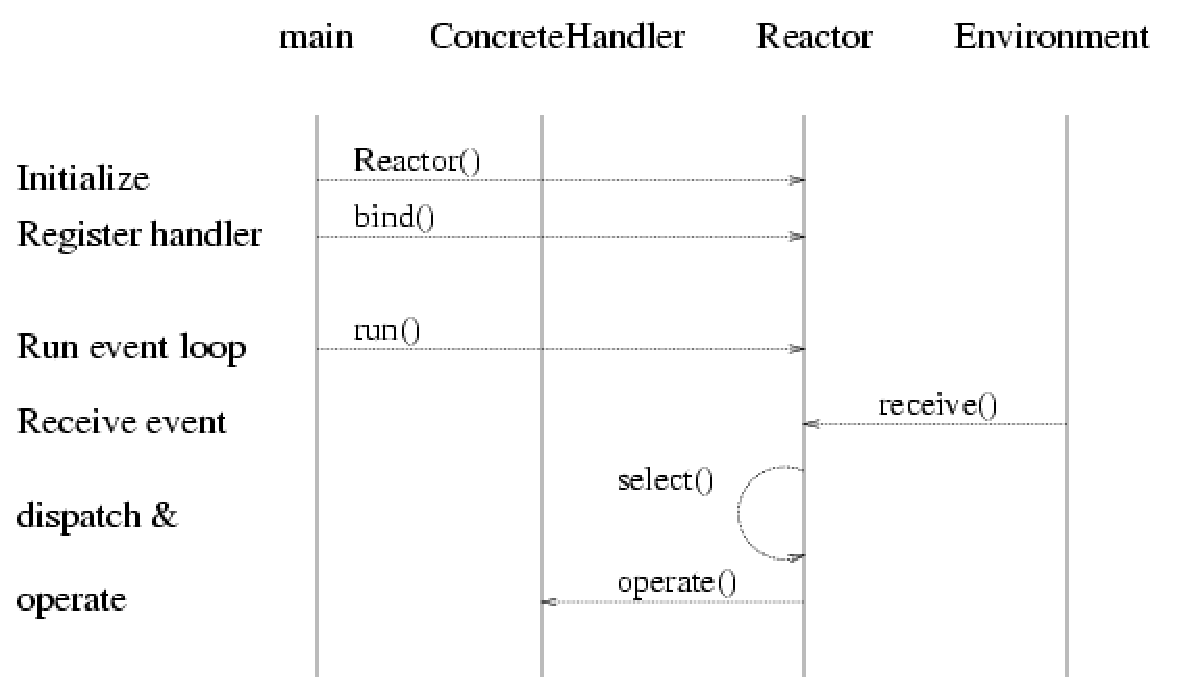
\includegraphics[scale=0.50]{figures/eventloop_flow.eps}
    \caption{The Sequence Diagram of the Reactor Model}
    \label{fig:eventloop_flow}
\end{figure}


\subsection{Reverse Proxy\\}

How it works, with more details.

\subsection{Message Queue\\}

Pub/Sub: with more details

Publisher: 

    * General design

    * Backend sever connect to the 

Subscriber: 

    * General Design

    * Client Design

    * Just 50 seconds

Message Management

Subscriber

Internal Data structure: what are the highlight of such design.

\subsection{Load Balancer\\}

HAProxy -- based on xxxx.

